\documentclass[a4paper, 12pt]{article}

%Абзацный отступ

\usepackage{indentfirst}

%Рисунки

\usepackage{graphicx}
\usepackage{wrapfig}

%Гиперссылки и работа с цветом

\usepackage{hyperref}
\usepackage[rgb]{xcolor}
\hypersetup{			%Гиперссылки
	colorlinks=true, 	%false: ссылки в рамках
	urlcolor=blue		%на URL
}

%Русский язык

\usepackage[T2A]{fontenc}		%кодировка
\usepackage[utf8]{inputenc}		%кодировка исходного текста
\usepackage[english, russian]{babel}	%локализация и переносы


%Математика

\usepackage{amsmath, amsfonts, amssymb, amsthm, mathtools, mathrsfs}

%Пакет с градусом

\usepackage{gensymb}

\author{Штрайх Роберт}
\title{Работа 3.4.2. Закон Кюри-Вейсса}
\date{05 октября 2021 г.}

\begin{document}
\begin{titlepage}
	\centering
	\vspace{5cm}
	{\scshape\LARGE Московский физико-технический институт \par}
	\vspace{4cm}
	{\scshape\Large Лабораторная работа №3.3.4 \par}
	\vspace{1cm}
	{\huge\bfseries Эффект Холла в полупроводниках \par}
	\vspace{1cm}
	\vfill
\begin{flushright}
	{\Large выполнил студент 006 группы ФЭФМ}\par
	\vspace{0.3cm}
	{\Large Штрайх Роберт}
\end{flushright}
	

	\vfill

% Bottom of the page
	Долгопрудный, 2021 г.
\end{titlepage}

\newpage

\textbf{Цель работы:} изучение температурной зависимости магнитной восприимчивости ферромагнетика выше точки Кюри.

\textbf{В работе используются:} катушка самоиндукции с образцом из гадолиния, термостат, частотомер, цифровой вольтметр, LC-автогенератор, термопара медь-константан.

\section{Теоретическое введение}

Вещества с отличными от нуля атомными магнитными моментами обладают парамагнитными свойствами. Внешнее магнитное поле ориентирует магнитные моменты, которые в отсутствие поля располагались в пространстве хаотичным образом.

При повышении температуры $ Т $ возрастает дезориентирующее действие теплового движения частиц, и магнитная восприимчивость парамагнетиков
убывает, в простейшем случае (в постоянном магнитном
поле) -- пo закону Кюри.

Для парамагнитных веществ, которые при понижении температуры становятся ферромагнитными, закон должен быть изменён. Температура $T = 0$ является особой точкой температурной кривой, в которой $\chi$ неограниченно возрастает. При $T \to 0$ тепловое движение всё меньше препятствует магнитным моментам атомов ориентироваться в одном направлении при сколь угодно слабом внешнем поле. В ферромагнетиках -- под влиянием обменных сил -- это происходит при понижении температуры не до абсолютного нуля, а до температуры Кюри $\theta$. У ферромагнетиков закон Кюри должен быть заменён законом Кюри-Вейсса:

\begin{equation}
\label{Кюри-Вейсс}
\chi\sim\frac{C}{T}\sim\frac{1}{T-\theta_p}, 
\end{equation}
где $\theta_p$ -- температура, близкая к температуре Кюри,
$C$ -- постоянная Кюри.

Эта формула хорошо описывает поведение ферромагнитных веществ после их перехода в парамагнитную фазу при заметном удалении температуры от $\theta$, но недостаточно точна при $T\approx\theta$.

В нашей работе изучается температурная зависимость $\chi(T)$ гадолиния при температуре выше точки Кюри. Выбор материала определяется тем, что его точка Кюри лежит в интервале комнатных температур.

\newpage

\section{Экспериментальная установка}

\begin{figure}[h]
\begin{center}
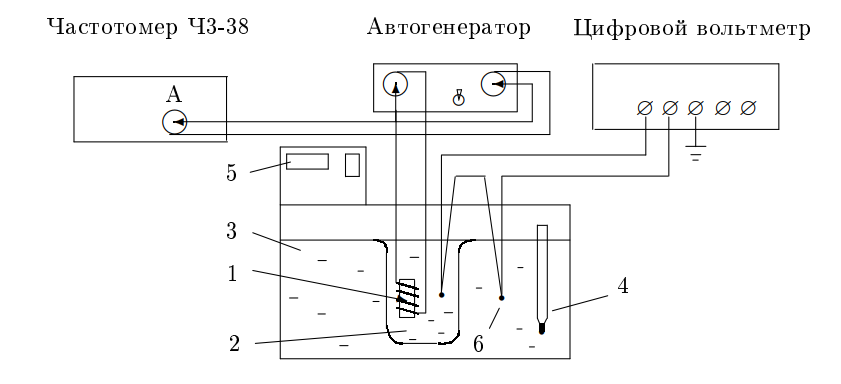
\includegraphics[width=1\textwidth]{Схема_установки}
\end{center}
\caption{Схема экспериментальной установки} \label{Установка}
\end{figure}

Схема установки для проверки закона Кюри-Вейсса показана на рис. \ref{Установка}. Исследуемый ферромагнитный образец (гадолиний) расположен внутри пустотелой катушки самоиндукции, которая служит индуктивностью, входящего в состав \textit{LC}-автогенератора. Катушка с образцом помещена в стеклянный сосуд, залитый трансфорамотрным маслом. Температура образца регулируется с помощью термостата.

При измененеии температуры по закону Кюри-Вейсса изменяется магнитная восприимчивость образца в катушке, и, следовательно, изменяется самоиндуктивность этой катушки. При этом изменяется период колебаний автогенератора:

\begin{equation}
\label{t}
\tau = 2\pi\sqrt{LC},
\end{equation}
где $C$ -- ёмкость контура автогенератора.

Период колебаний в отсутствие образца определяется самоиндукцией пустой катушки:

\begin{equation}
\label{t0}
\tau_0 = 2\pi\sqrt{L_0C},
\end{equation}

Из (\ref{t}) и (\ref{t0}) имеем

\begin{equation}
\label{Соотношение}
\frac{1}{\chi}\sim(T-\theta_p)\sim\left(\frac{1}{\tau^2-\tau_0^2}\right).
\end{equation}

Измерения проводятся в интервале температур от 14 $\degree$C до 40 $\degree$C.

\section{Ход работы}

\begin{enumerate}

\item Оценим допустимую ЭДС термопары при допустимой разности температур и рабочей жидкости $\Delta T = 0,5\degree$C, постоянная термопары $k = 24$ град/мВ:

\[\mathscr{E} = k \cdot \Delta T = 0,02 \text{ мВ},\]

\item Зафиксируем период колебаний без образца $\tau_0 = 6,909$ мкс.

Исследуем зависимость периода колебаний \textit{LC}-генератора от температуры образца, отмечая период колебаний $\tau$ по частотомеру, а температуру $T$ -- по показаниям дисплея и цифровому вольтметру. Результаты измерений занесём в таблицу \ref{Period_table} и построим по ним график (рис. \ref{Period_graph})

\begin{table}[h]
\caption{Зависимость периода колебаний в генераторе от температуры образца}
\small
\begin{tabular}{|l|l|l|l|l|l|l|l|l|l|l|l|l|l|l|}
\hline
$T, \degree$\textit{С}                       & 13,2   & 15     & 17     & 19     & 21     & 23     & 25     & 27     & 29     \\ \hline
$T_{real}, \degree$\textit{C}                  & 13,68  & 15,48  & 17,48  & 19,48  & 21,48  & 23,48  & 25,48  & 27,48  & 29,48  \\ \hline
$\tau$, \textit{мкс}                     & 7,97   & 7,927  & 7,844  & 7,707  & 7,515  & 7,306  & 7,182  & 7,127  & 7,094  \\ \hline
\textit{$\frac{1}{(\tau^2-\tau_0^2)}$, мкс$м^{-2}$} & 0,0633 & 0,0662 & 0,0725 & 0,0857 & 0,1144 & 0,1772 & 0,2600 & 0,3268 & 0,3860 \\ \hline
\hline
$T, \degree$\textit{С}                                                              & 31     & 33     & 35     & 37     & 39    & & & &\\ \hline
$T_{real}, \degree$\textit{C}                                    & 31,48  & 33,48  & 35,48  & 37,48  & 39,48 & & & & \\ \hline
$\tau$, \textit{мкс}                                      & 7,071  & 7,055  & 7,043  & 7,034  & 7,026 & & & &\\ \hline
\textit{$\frac{1}{(\tau^2-\tau_0^2)}$, мкс$м^{-2}$} & 0,4415 & 0,4905 & 0,5349 & 0,5738 & 0,6133 & & & &\\ \hline

\end{tabular}
\label{Period_table}
\end{table}

\item Прямую ферромагнитного участка экстраполируем к оси абсцисс, полученное значение -- экспериментальное значение точки Кюри для исследуемого образца Гадолиния.

Учтём погрешности приборов, погрешность поддержания температуры термостатом -- 0,01 $\degree$C; погрешность термопары (в градусах) -- 0,28 $\degree$C.
 
Полученное значение:

\[\theta_p = (14,1\pm0,3)\degree C\]

Табличное значение: 20,2 $\degree$C

\end{enumerate}

\section{Выводы}

В ходе работы мы определили парамагнитную точку Кюри для гадолиния, исследован переход от ферромагнитного к парамагнитному состоянию.

\begin{itemize}
\item Экспериментальное значение точки Кюри:

\[\theta_p = (14,1\pm0,3)\degree C,\]
\[\varepsilon_{\theta_p} = 2,04 \text{\%},\]

\item Табличное значение точки Кюри $\theta_{theor} = 20,2 \degree C.$

Табличное и экспериментальное значения несколько отличаются друг от друга, однако данный метод измерения лучше подходит для веществ, у которых точка Кюри находится в интервале комнатных температур.
\end{itemize}

\newpage
\section{Приложение}

\begin{figure}[h]
\begin{center}
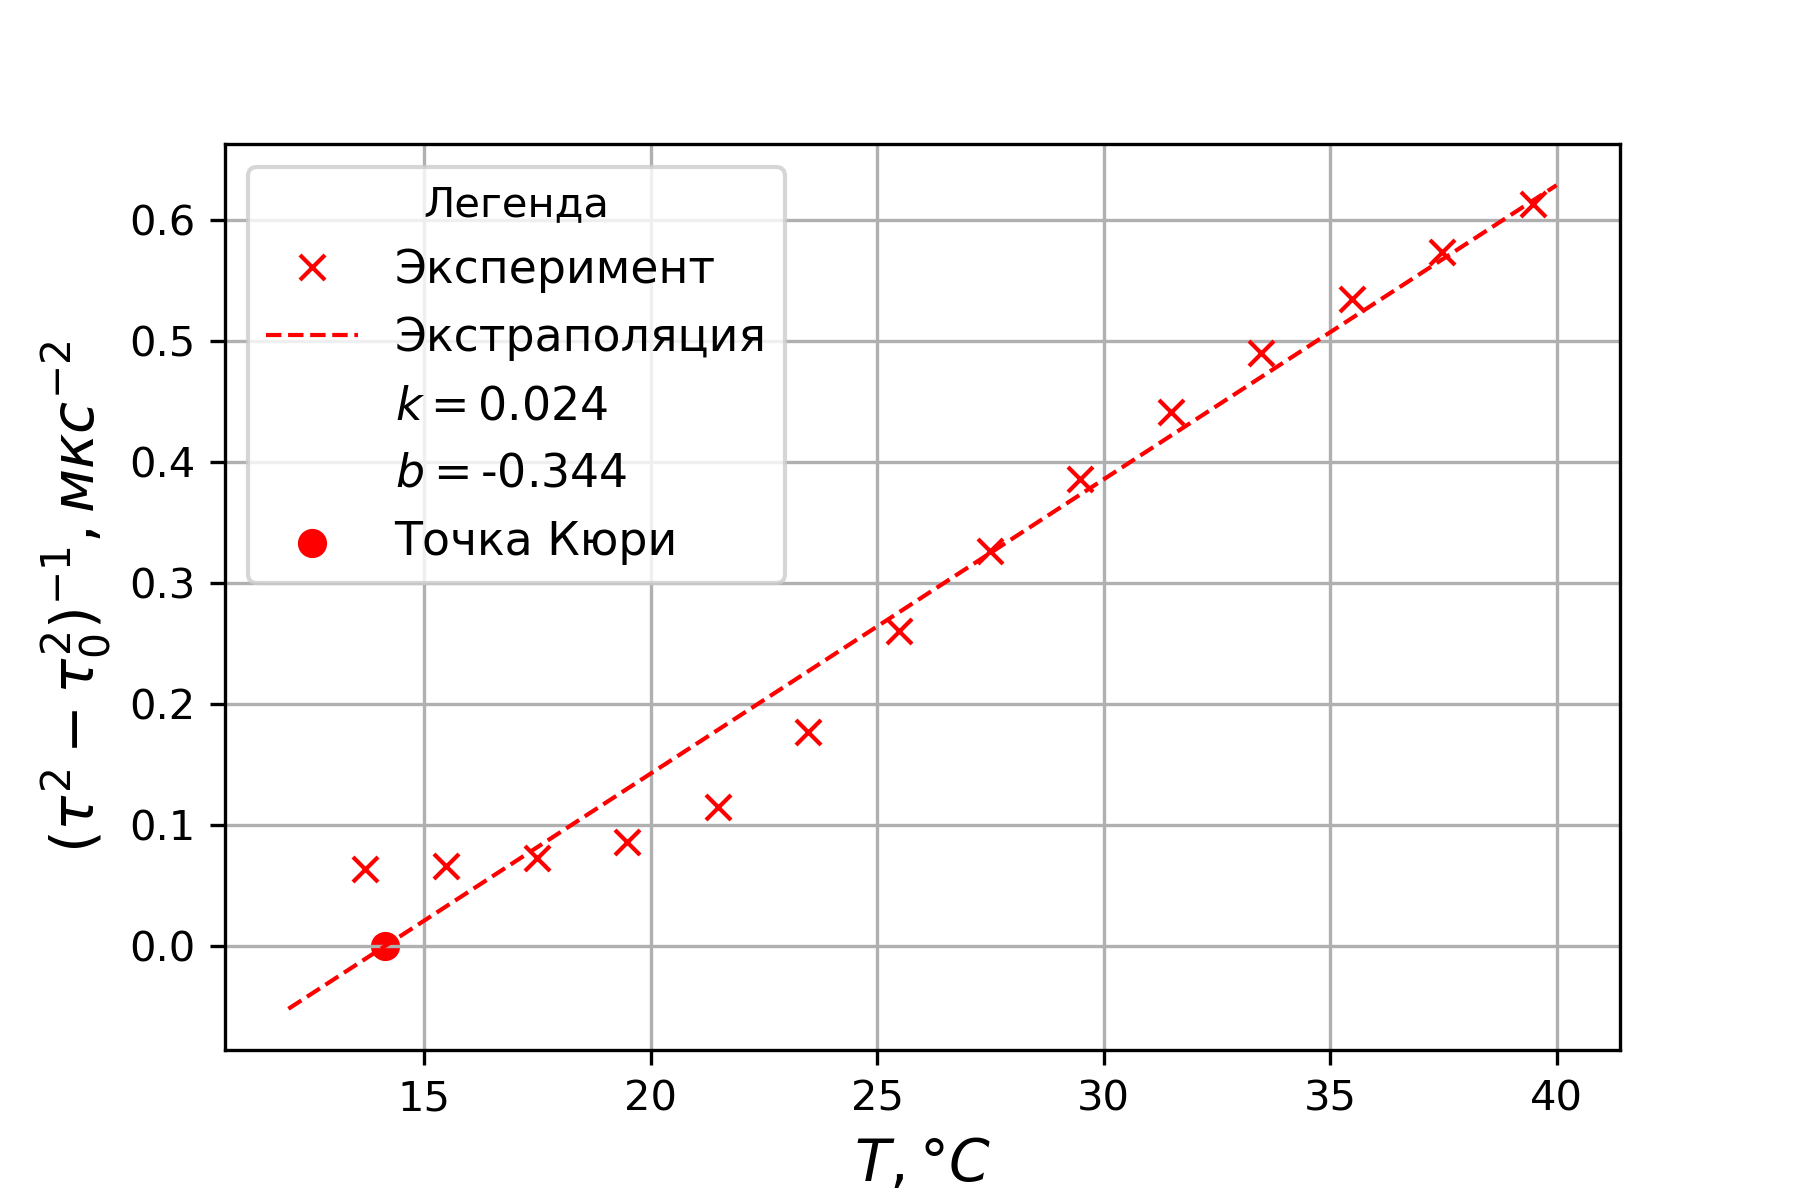
\includegraphics{graph.png}
\end{center}
\caption{$1/(\tau^2-\tau_0^2) = f(T)$}
\label{Period_graph}
\end{figure}

\begin{figure}[h]
\begin{center}
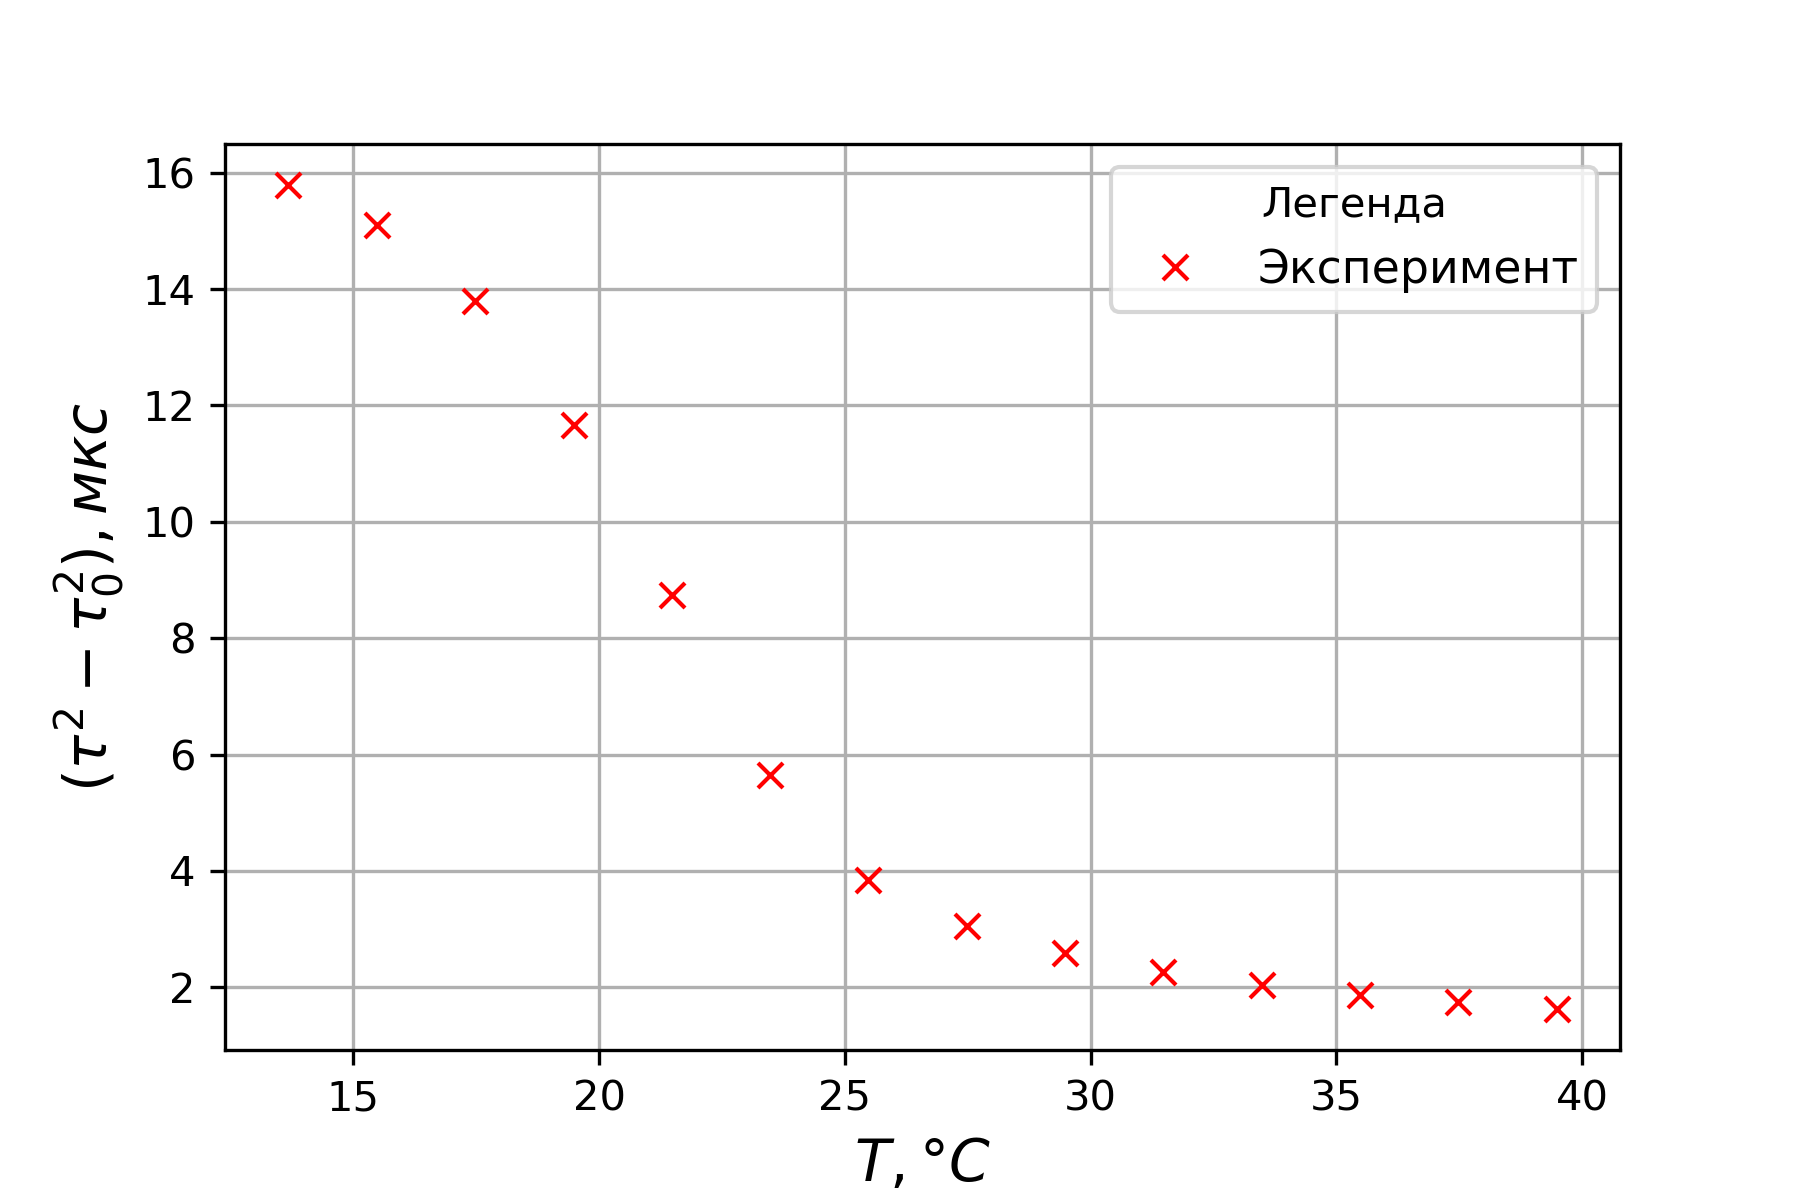
\includegraphics{graph1.png}
\end{center}
\caption{$\tau^2-\tau_0^2 = f(T)$}
\label{Period_graph1}
\end{figure}

\end{document}